\documentclass[draft ]{article}
\usepackage[utf8]{inputenc}

\title{science-article-2}
\author{lorenzo.versini }
\date{December 2019}

%\usepackage{natbib}
%\usepackage{cite}
\usepackage[sorting=none]{biblatex}
\bibliography{references}
\usepackage{graphicx}
\usepackage[most]{tcolorbox}
\usepackage{xcolor,sectsty}

\usepackage{subcaption}
\hyphenation{op-tical net-works semi-conduc-tor am-pe-ro-me-ter de-mon-stra-te He-nce me-et a-ga-in spea-ches}

\usepackage[width=14cm, left=2cm]{geometry}

\definecolor{astral}{RGB}{46,116,181}
\subsectionfont{\color{astral}}
\sectionfont{\color{astral}}

\tcbset{enhanced,colback=astral!5!white, boxrule=0.4pt,sharp corners, colframe=astral!75!black,fonttitle=\bfseries}

\begin{document}
\twocolumn
\maketitle

\section{Introduction}


Whisper in an open green field and nobody will hear you. Whisper in St. Paul Whispering Gallery (London) and people at 30m distance will be able to listen to you.

It is obvious that a great contribution to how we perceive sound is given by the surrounding and the geometry of the system. The attempt to understand and exploit it to enhance sounds 

The question is, how exactly do spaces amplify sounds? What can we say about a particular concert hall? Is there a way we can objectively distinguish a good space from a bad one?

In order to address these points, we need first to understand what sound is and how it propagates through space.

\section{Pressure waves and whispering on Walls}

A sound wave is a pressure fluctuation in air \cite{book:university_physics} which travels in the medium with a speed in the order of 340 m/s.

It is described by the wave equation,

\begin{equation}
\frac{\partial^2 u}{\partial t^2} = c^2 \frac{\partial^2 u}{\partial x^2}
\end{equation}

and it has all the property of waves.
For instance, as a sound wave hits a surface, it is reflected as other waves do. Similarly to light, a ray approach can be used to describe the propagation of sound in a closed space, even though wavelengths are much bigger (the A note Orchestras tune on, has a wavelength of approx. 0.8m).

We all have the intuitive description that the further we go, the weaker the wave is: it is difficult to listen to someone speaking far from us when we are in a large open space.
Indeed, again similarly to the light from a star, sound waves follow a
\begin{equation}
\frac{1}{r^2}
\end{equation}

law, which means that if we double the distance, the amplitude of oscillation reduces by four.

Again, no surprise, when sound waves meet a surface, as a wall, they are partly reflected and partly absorbed, and this is where acoustic arises! By carefully shaping the geometry of a closed environment, very particular effects can be created.

An example is the Whispering gallery situated in St. Paul Cathedral (London) which is famous for the fact that if two people stand at opposite sides of the room along the wall, they can whisper each other and still listening what they are saying \cite{article:whispering}.

\begin{figure}[ht!]
\centering
\begin{tcolorbox}[drop lifted shadow]

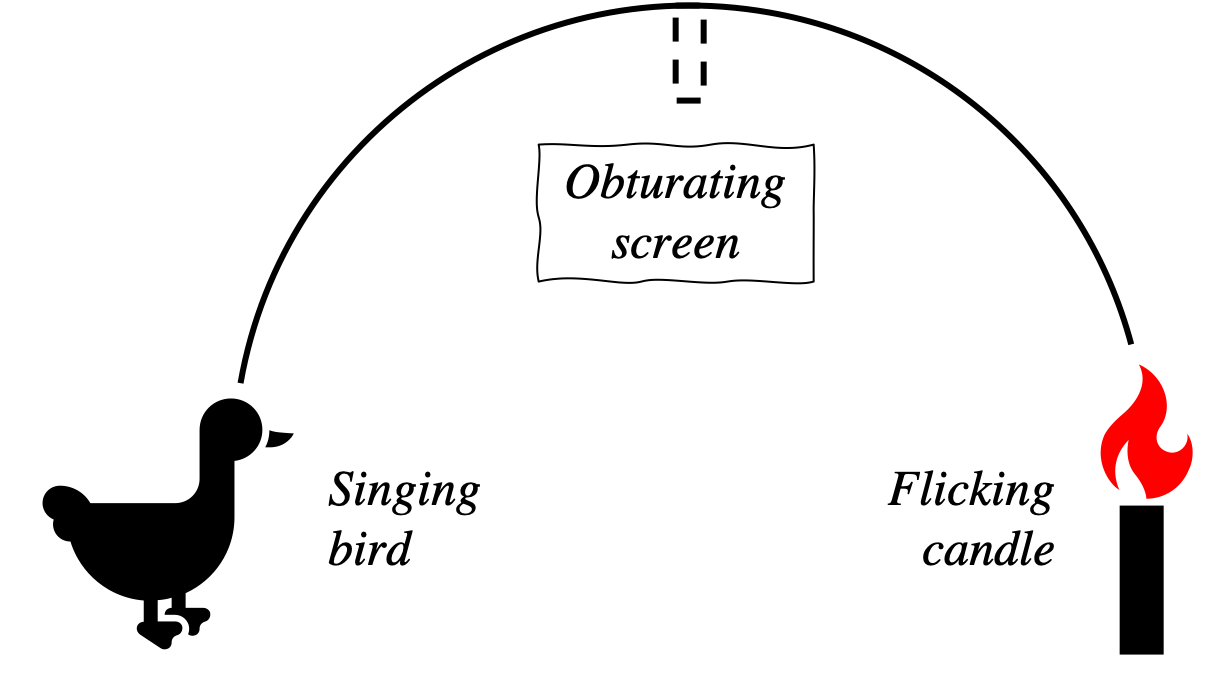
\includegraphics[scale=0.3]{rayleigh_experiment}
\caption{ Shows the experiment Rayleigh performed. A singing bird was firstly placed in front of a flicking candle at 2m and it was observed that no movement in the flame could be seen. Then the bird and the candle were placed inside a cylindrical metallic plate and the flame moved as the animal sang. Lastly, an obturating screen was placed along the metallic plate and the absence of movement in the flame showed that sound waves were propagating along the surface of the screen }
\label{fig:duck}

\end{tcolorbox}\par\bigskip
\end{figure}

Lord Rayleigh (some info about him) in 1896 proposed an explanation for this phenomenon which agrees with numerical and physical tests.

The idea is that sound waves would reflect and propagate along the surface of the wall, finally reaching the person on the other side.

He performed a simple experiment to demonstrate his hypothesis. He placed a bird and a flame at a distance of 2m one from the other and noticed that when the bird sang, no flickering in the flame could be noticed ()

Then he placed bird and flame in a cylindrical metallic plate of diameter of 2 meters at the same distance and noticed that as the bird sang, the flame started to fickle.
Lastly, he used an obturating screen to obstruct the way along the inner surface of the cylinder and noticed that this time the flame did not fickle. \cite{article:whispering}

This enforced the idea that because of the circular geometry, sound waves propagated along the walls, allowing less energy losses and thus explaining the peculiarities of architectural structures.

\section{Interpreting Judgments}
If you ask a professional musician to play in a room and then to judge the quality of the acoustic, he will come out with some bizarre words like, dry, or full.

Then, if you ask another musician, there is a good chance that he will independently agree with the other’s opinion. Therefore, there must be some physical effect, something which makes a room’s sound dry.

However, in order to define that, we need to understand what dry scientifically means! This was done by comparing people’s judgments with room’s measured parameters for a variety of different architectural spaces.
Hence, a bridge between what are subjective parameters and objective parameters was built. [3]

\section{Reverberance}
A main parameter is reverberance. The word comes from the prefix “re-” which means again and the latin “verberare” i.e. to whip [4]. Cambridge Dictionary defines it as the quality of a sound that lasts for long and makes things vibrate.

What causes a sound to last in a room even if the sound source has been shut?

\begin{figure}[ht!]
\centering
\begin{tcolorbox}[drop lifted shadow]

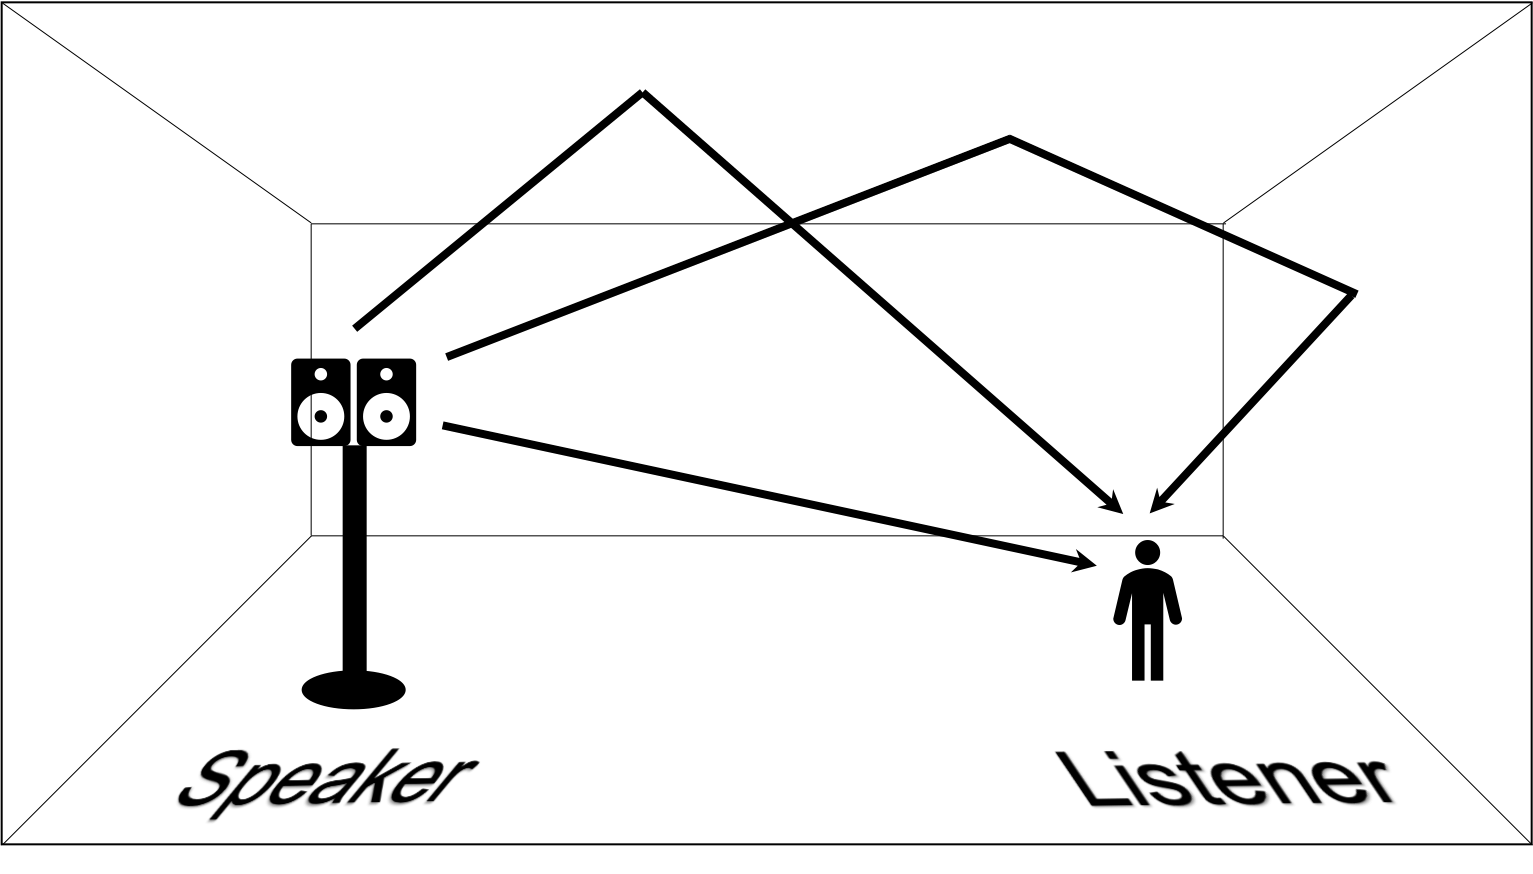
\includegraphics[scale=0.22]{reverberant-box}
\caption{Schematic representation of a room. Sound from the speaker reaches the listener at different times, causing the sound level to increase over time}
\label{fig:box}

\end{tcolorbox}\par\bigskip
\end{figure}

Let's analyse the scenario represented in Fig. \ref{fig:box}, where a speaker produces a sound in a room and there is a listener. Firstly, he is reached by the direct sound (ray \textbf{A}), then all the other reflections reach him at following times (i.e. \textbf{B}, \textbf{C}).

Therefore, the sound level as perceived by the listener increases over time. Eventually, an equilibrium is reached between the speaker continuing adding energy as sound waves and the absorption of air and surfaces (e.g. walls) and a constant intensity is reached.

Similarly, as the source is suddenly shut, the intensity level takes time to decrease, as all the energy stored as sound waves needs to be absorbed or dispersed. 

This process requires time according to the absorption coefficients of the surfaces in the room. If the sound stays for long, then we say that the room is reverberant.

Hence, it seems natural that a way to characterise the reverberance of a closed space, we could measure how long a sound stays a room after the source was shut.

The actual definition of the \textit{reverberation time} involves the intensity of a sound $L_I$ i.e. the logarithm,

\begin{equation}
L_I = 10 \log_{10}{\frac{I}{I_0}}\ \mathrm{dB}
\end{equation}

where $I_0$ is a reference value and it is the lowest intensity that an average person can perceive at $1000\ \mathrm{Hz}$ \cite{book:acoustic2}.

Then, the reverberation time is defined as the time that it takes to the sound in a room to decrease by $60$ decibels after shutting down the source. In practice, the drop time is evaluated between $-5 \mathrm{dB}$ and $-35 \mathrm{dB}$ as follows,

\begin{equation}
T = 60 \mathrm{dB} \frac{t_{-35} - t_{-5}}{(-5\mathrm{dB}) - (-35\mathrm{dB})}
\end{equation}

Two good reasons why the reverberation time is evaluated according to a logarithmic scale rather than a linear one are that the intensity level is a scale which better approximates the way we perceive sound \cite{book:acoustic2} and that we expect the intensity fall to be exponential-like \cite{book:acoustic}.

\subsection{Speaches and Music}


\printbibliography

%\bibliographystyle{plain}
%\bibliography{IEEEabrv,references}
\end{document}
